\documentclass[12pt,a4paper,portuguese]{article}
\usepackage[T1]{fontenc}
\usepackage{babel}
\usepackage{graphicx}
\usepackage{float}
\usepackage{pythonhighlight}

\title{Lista 5 - Análise de Séries Temporais em Oceanografia}
\author{Lucas Salimene}
\date{}
\begin{document}
	\maketitle
	\newpage
	\textbf{Parte I – Série de Fourier}
	
	Visualizando as séries temporais conforme ilustrado na figura
	
\begin{figure}[H]
	\centering
	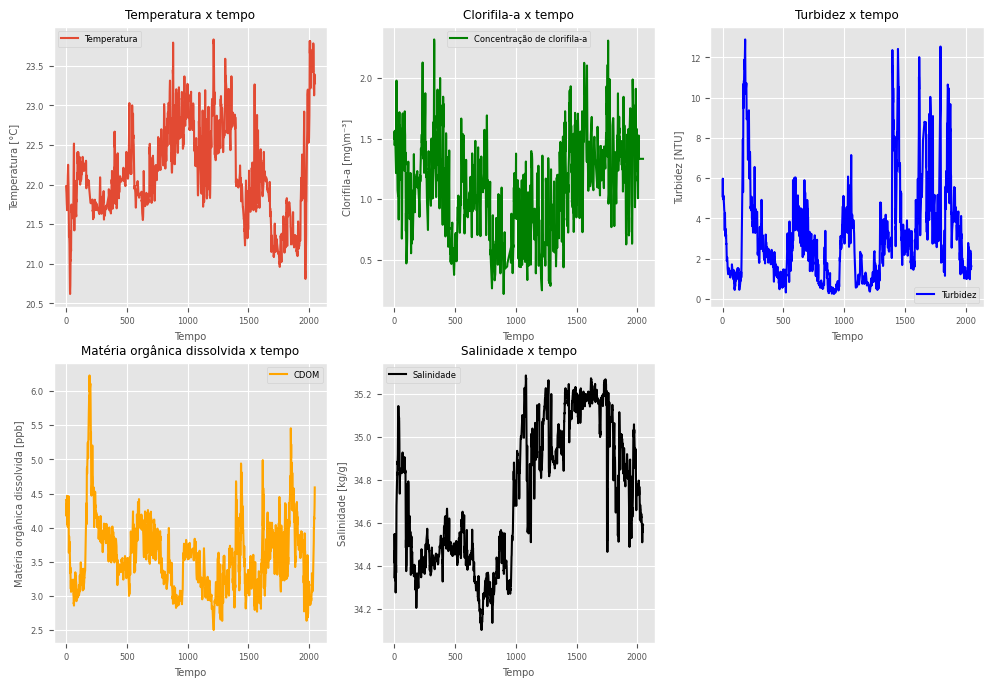
\includegraphics[width=1\linewidth]{lista5-1b}
	\caption{Variáveis disponível na série temporal}
	\label{fig:lista5-1b}
\end{figure}

Calculando a PSD com a função welch do pacote SciPy para as altas e baixas frequências conforme ilustrado nas figuras \ref{fig:lista5-2c} e \ref{fig:lista5-2d} respectivamente
	\begin{figure}[H]
		\centering
		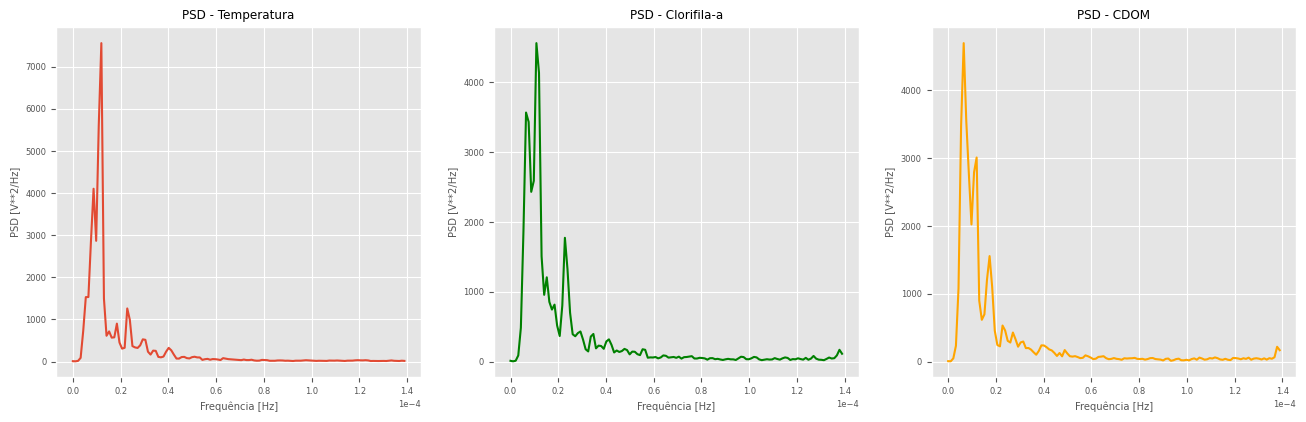
\includegraphics[width=1\linewidth]{lista5-2c}
		\caption{Densidade espectral de potência (PSD) para as altas frequências das variáveis de temperatura, clorofila e concentração de matéria orgânica dissolvida (CDOM) }
		\label{fig:lista5-2c}
	\end{figure}
		\begin{figure}[H]
		\centering
		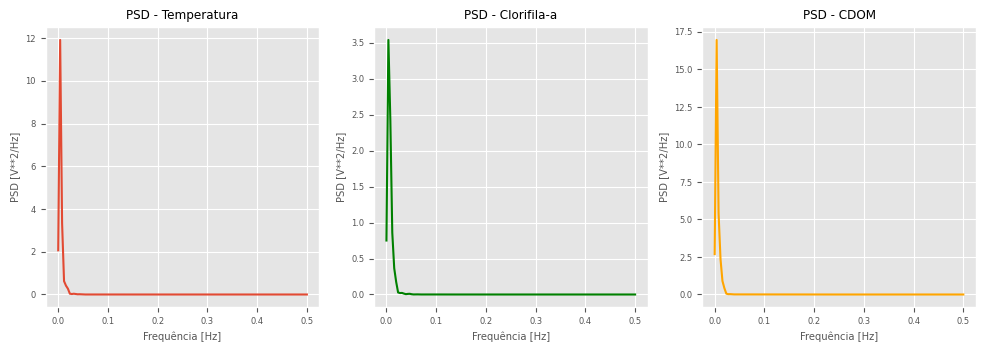
\includegraphics[width=1\linewidth]{lista5-2d}
		\caption{Densidade espectral de potência (PSD) para as baixas frequências das variáveis de temperatura, clorofila e concentração de matéria orgânica dissolvida (CDOM) }
		\label{fig:lista5-2d}
	\end{figure}
	
\textbf{Parte II – Análises Espectrais utilizando os métodos de Welch e Lamb}

Plotando a densidade espectral de potência para a série disponível em \textit{freqanal.dat}, se obtém a figura \ref{fig:lista5-3a}.

	\begin{figure}[H]
	\centering
	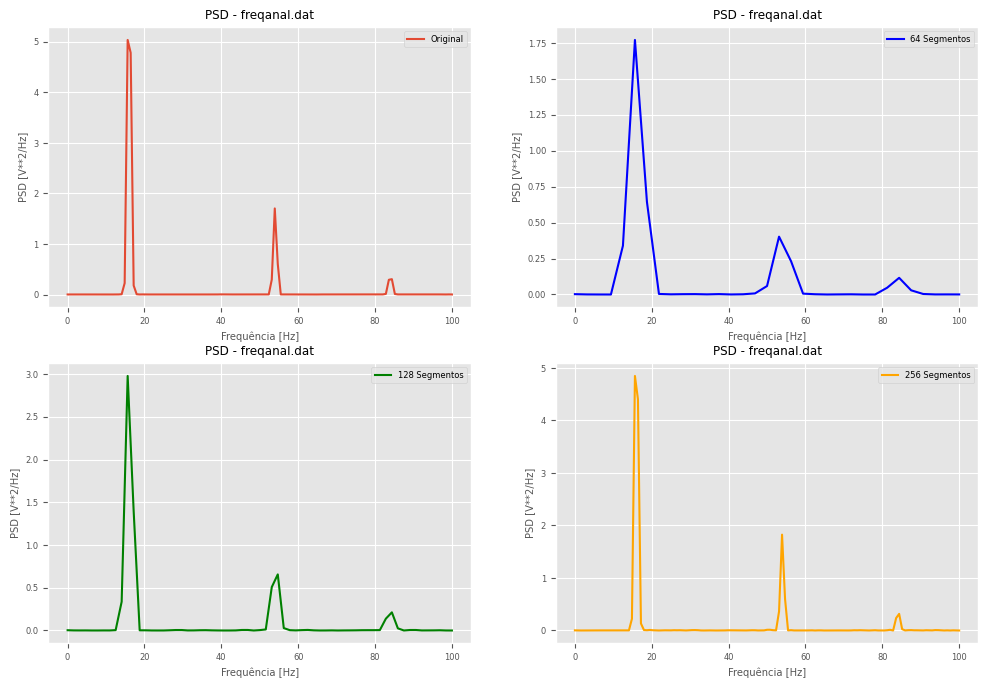
\includegraphics[width=1\linewidth]{lista5-3a}
	\caption{Densidade espectral de potência (PSD) para a série do dado \textit{freqanal.dat} com diferentes segmentos }
	\label{fig:lista5-3a}
\end{figure}

Adicionando uma frequência adicional de 110Hz se obtêm a figura  \ref{fig:lista5-3b}.

\begin{figure}[H]
	\centering
	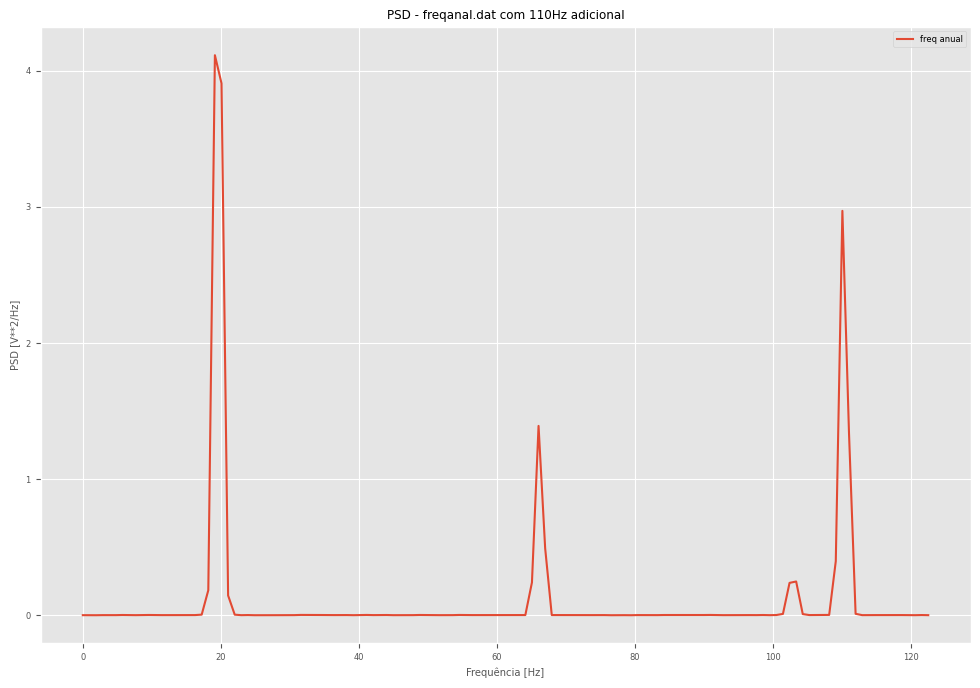
\includegraphics[width=1\linewidth]{lista5-3b}
	\caption{Densidade espectral de potência (PSD) para a série do dado \textit{freqanal.dat} com  uma frequência adicional de 110Hz }
	\label{fig:lista5-3b}
\end{figure}


Os histogramas dos arquivos \textit{fu.dat} e \textit{tu.dat} são apresentadas na figura \ref{fig:lista5-4a}.

\begin{figure}[H]
	\centering
	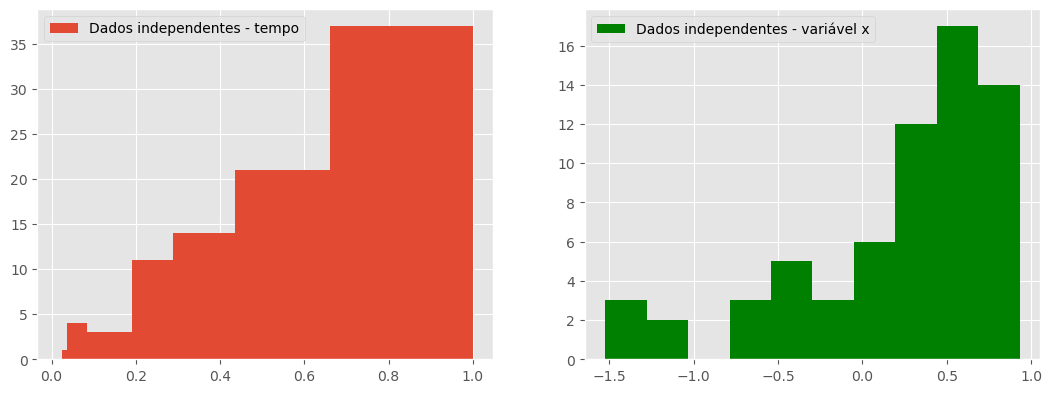
\includegraphics[width=1\linewidth]{lista5-4a}
	\caption{Histogramas dos arquivos \textit{fu.dat} e \textit{tu.dat}}
	\label{fig:lista5-4a}
\end{figure}

Utilizando o pacote SciPy para calcular a PSD pelo método de Lamb, se obtém a figura \ref{fig:lista5-4b}.

\begin{figure}[H]
	\centering
	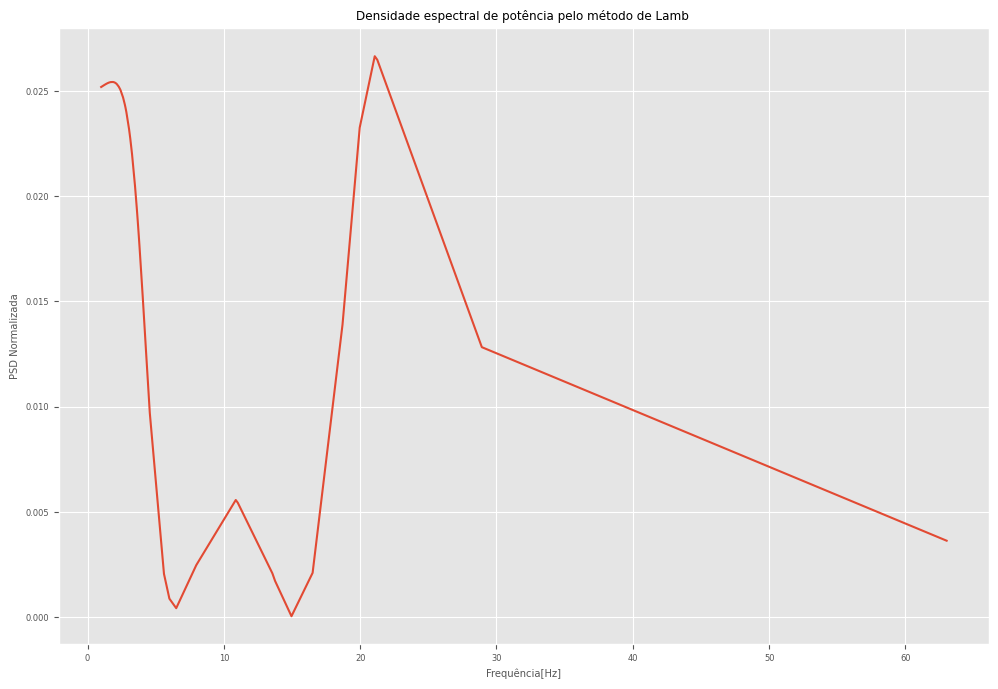
\includegraphics[width=1\linewidth]{lista5-4b}
	\caption{PSD pelo método de Lamb dos arquivos \textit{fu.dat} e \textit{tu.dat}}
	\label{fig:lista5-4b}
\end{figure}
Com as frequências dominantes sendo as de 0Hz e a de 20Hz.

\end{document}